\documentclass[10pt]{article}

% Packages pour les marges
\usepackage[
    top=2cm,
    bottom=2cm,
    left=2cm,
    right=2cm
]{geometry}

% Police sans serif
% \usepackage{helvet}
% \renewcommand{\familydefault}{\sfdefault}

% Packages existants
\usepackage[french]{babel}
\usepackage[utf8]{inputenc}
\usepackage[T1]{fontenc}
\usepackage{amsmath}
\usepackage{amsfonts}
\usepackage{amssymb}
\usepackage[version=4]{mhchem}
\usepackage{stmaryrd}
\usepackage{listings}

\usepackage{enumitem}
\usepackage{ifthen}
\usepackage{graphicx}
\usepackage{verbatim}
\usepackage{url}
\usepackage{mdframed}
\usepackage[sf]{titlesec}
\titleformat{\section}{\sffamily\large\bfseries}{\thesection}{1em}{}
% Définition de la variable pour afficher les corrections
\newboolean{showSolutions}
% Décommentez la ligne suivante pour afficher les solutions
\input \jobname.adr
% \input \jobname.adr


\title{TD0 - Analyse Numérique}

\author{}
\date{}

\newenvironment{solution}
    {\par\vspace{0.5em}\begin{mdframed}[linewidth=0.5pt]\par}
    {\end{mdframed}\par\vspace{0.5em}}

\begin{document}
\sffamily
\maketitle
\vspace{1cm}
\section*{Manipulations d'erreurs}

On donne les première décimales de $\pi$ : $3.14159\cdots$.

Quelle erreur fait-on lorsqu'on approche la valeur de $\pi$ par $3.14$ ? \newline
\noindent On calculera l'erreur absolue et l'erreur relative.

\ifthenelse{\boolean{showSolutions}}{
\begin{solution}
    \begin{align*}
        \text{Erreur absolue} &= |\pi - 3.14| \approx 0.00159 \approx 10^{-3}
    \end{align*}
    C'est donc une valeur approchée de $\pi$ à $10^{-3}$ près.
    \begin{align*}
        \text{Erreur relative} &= \frac{|\pi - 3.14|}{\pi} = \frac{0.00159}{3.14159} \approx 0.000506 \approx 0.05\%\,.
    \end{align*}
    En remplaçant $\pi$ par $3.14$ on commet une erreur relative de $0.05\%$.
\end{solution}
}{}
\vspace{2cm}

\section*{Une suite récurrente}
\begin{enumerate}
\item Pour calculer la valeur de $\sqrt{2}$, on utilise la suite récurrente :
\begin{align*}
    \left\{
    \begin{array}{l}
        x_0 = 1 \\
        x_{n+1} = \frac{x_n + \frac{2}{x_n}}{2}
    \end{array}
    \right.
\end{align*}
Listez les $3$ premiers termes de la suite. 

\ifthenelse{\boolean{showSolutions}}{
\begin{solution}
    $x_0 = 1$
    $x_1 = \frac{1 + \frac{2}{1}}{2} = 1.5$
    $x_2 = \frac{1.5 + \frac{2}{1.5}}{2} \approx 1.417$
\end{solution}
}{}

\item Quelle est la fonction $f$ qui permet d'écrire $x_{n+1} = f(x_n)$ ?

\ifthenelse{\boolean{showSolutions}}{
\begin{solution}
    \begin{align*}
        f(x) = \frac{1}{2}\Big(x + \frac{2}{x}\Big)\,.
    \end{align*}
\end{solution}
}{}

\item Vérifier que $f$ est contractante sur l'intervalle $[1, 2]$. \textit{Ce qui signifie que $|f'|<1$, on pourra remarquer que $f'$ est croissante. }. 

\ifthenelse{\boolean{showSolutions}}{
\begin{solution}
    On calcule la dérivée de $f$ :
    \begin{align*}
        f'(x) = \frac{1}{2}\Big(1 - \frac{2}{x^2}\Big)
    \end{align*}
    $f'$ croît mais n'est pas de signe constant donc $f' < \max\big(|f'(1)|, |f'(2)|\big)=\max\big(\frac{1}{2}, \frac{1}{4}\big)=\frac{1}{2} < 1$
\end{solution}
}{}

\item Quel théorème du cours permet de conclure que la suite $(x_n)$ converge vers $\sqrt{2}$ ?

\ifthenelse{\boolean{showSolutions}}{
\begin{solution}
    Le théorème du point fixe.
\end{solution}
}{}

\item Calculer avec une calculatrice les 4 premières itérations de la suite $(x_n)$ en partant de $x_0 = 1$. \newline
\noindent Quelle erreur commet-on en prenant $x_3$ comme approximation de $\sqrt{2}$ ?

\ifthenelse{\boolean{showSolutions}}{
\begin{solution}
    $x_0 = 1$
    $x_1 = 1.5$
    $x_2 \approx 1.417$
    $x_3 \approx 1.414216$

    Des méthodes plus élaborées comme celle qu'utilise la calculatrice donnent $\sqrt{2} \approx 1.414213\cdots$. 
    L'erreur commise est donc de $10^{-6}$ environ. L'erreur relative de $10^{-6}/\sqrt{2} \approx 0.0001\%$ environ.
\end{solution}
}{}

\item Rédiger un pseudo code pour calculer $x_{100}$. 

\ifthenelse{\boolean{showSolutions}}{
\begin{solution}
    x = 1

    Pour i allant de 1 à 100:

    \hspace{2em}    x = (x + 2/x) / 2

    Afficher x

\end{solution}
}{}

\end{enumerate}
\vspace{2cm}
\section*{Dichotomie}
On considère l'équation $xe^x = 1$.
\begin{enumerate}
\item Tracer des graphes de fonctions bien choisies pour vous convaincre qu'il existe une unique solution positive à cette équation. Et déterminer un intervalle de longueur $1$ dans lequel se trouve cette solution. 

\ifthenelse{\boolean{showSolutions}}{
\begin{solution}
    On trace les fonctions $f(x)=e^x$ et $g(x)=1/x$,la solution se trouve au point d'intersection de ces deux courbes. 
\begin{center}
    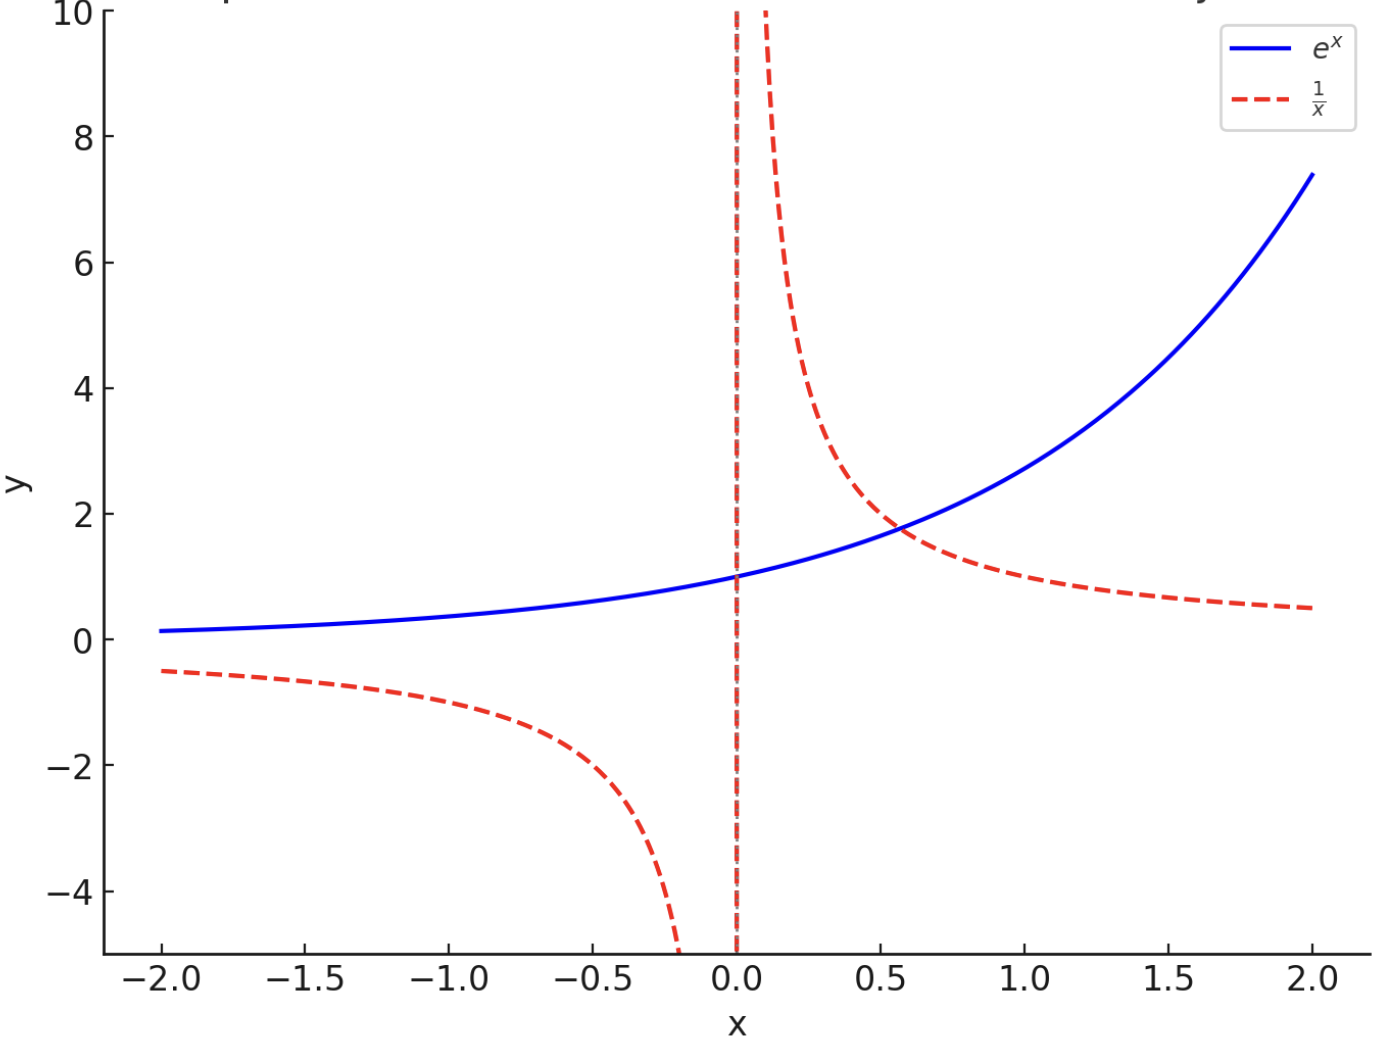
\includegraphics[width=0.5\textwidth]{graphes.png}
\end{center}
\end{solution}
}{}

\item On veut approcher cette solution par la méthode de dichotomie. Indiquez les premières étapes de l'algorithme. 

\ifthenelse{\boolean{showSolutions}}{
\begin{solution}
    On définit la fonction 
    \[
        f(x) = xe^x - 1
    \]
    \begin{itemize}
        \item La solution se situe entre $0.2$ et $0.8$ environ.
        \item On essaie la valeur entre les deux : $0.5$. 
        \[
            f(0.5) \approx -0.18 < 0
        \]
        donc la solution est entre $0.5$ et $0.8$.
        \item On essaie la valeur $0.65$ : $f(0.65) \approx 0.245 > 0$ donc la solution est entre $0.5$ et $0.65$.
        \item On essaie la valeur $0.575$ : $f(0.575) \approx 0.02 > 0$ donc la solution est entre $0.575$ et $0.65$.
    \end{itemize}

\end{solution}
}{}

\item Rédiger un pseudo-code pour implémenter la méthode. 

\ifthenelse{\boolean{showSolutions}}{
\begin{solution}
    a = 0.2

    b = 0.8

    Tant que  b - a > 1e-10:

      \hspace{2em}  m = (a + b) / 2

      \hspace{2em}  Si f(m) < 0

       \hspace{2em}\hspace{2em}     a = m

       \hspace{2em} Sinon

        \hspace{2em}\hspace{2em}    b = m

    Afficher m
\end{solution}
}{}


\item Combien d'opérations sont nécessaires pour approcher la solution à $10^{-10}$ près ?

\ifthenelse{\boolean{showSolutions}}{
\begin{solution}
    On fait $n$ itérations, à chaque fois la longueur de l'intervalle est divisée par $2$ on cherche $n$ tel que  
    \[
        \frac{b-a}{2^n} = 10^{-10}\,. 
    \]
    Donc $n$ doit dépasser 
    \[
        \log_2\Big((b-a)10^{10}\Big) \approx 32.5
    \]
    soit $33$ itérations.
\end{solution}
}{}

\end{enumerate}

\newpage

\section*{Méthode de Newton}
On considère la fonction $f(x) = x^2-3$.
\begin{enumerate}
\item Tracer le graphe de $f$ et la tangente à $f$ en $x=2$. 

\ifthenelse{\boolean{showSolutions}}{
\begin{solution}
    \begin{center}
        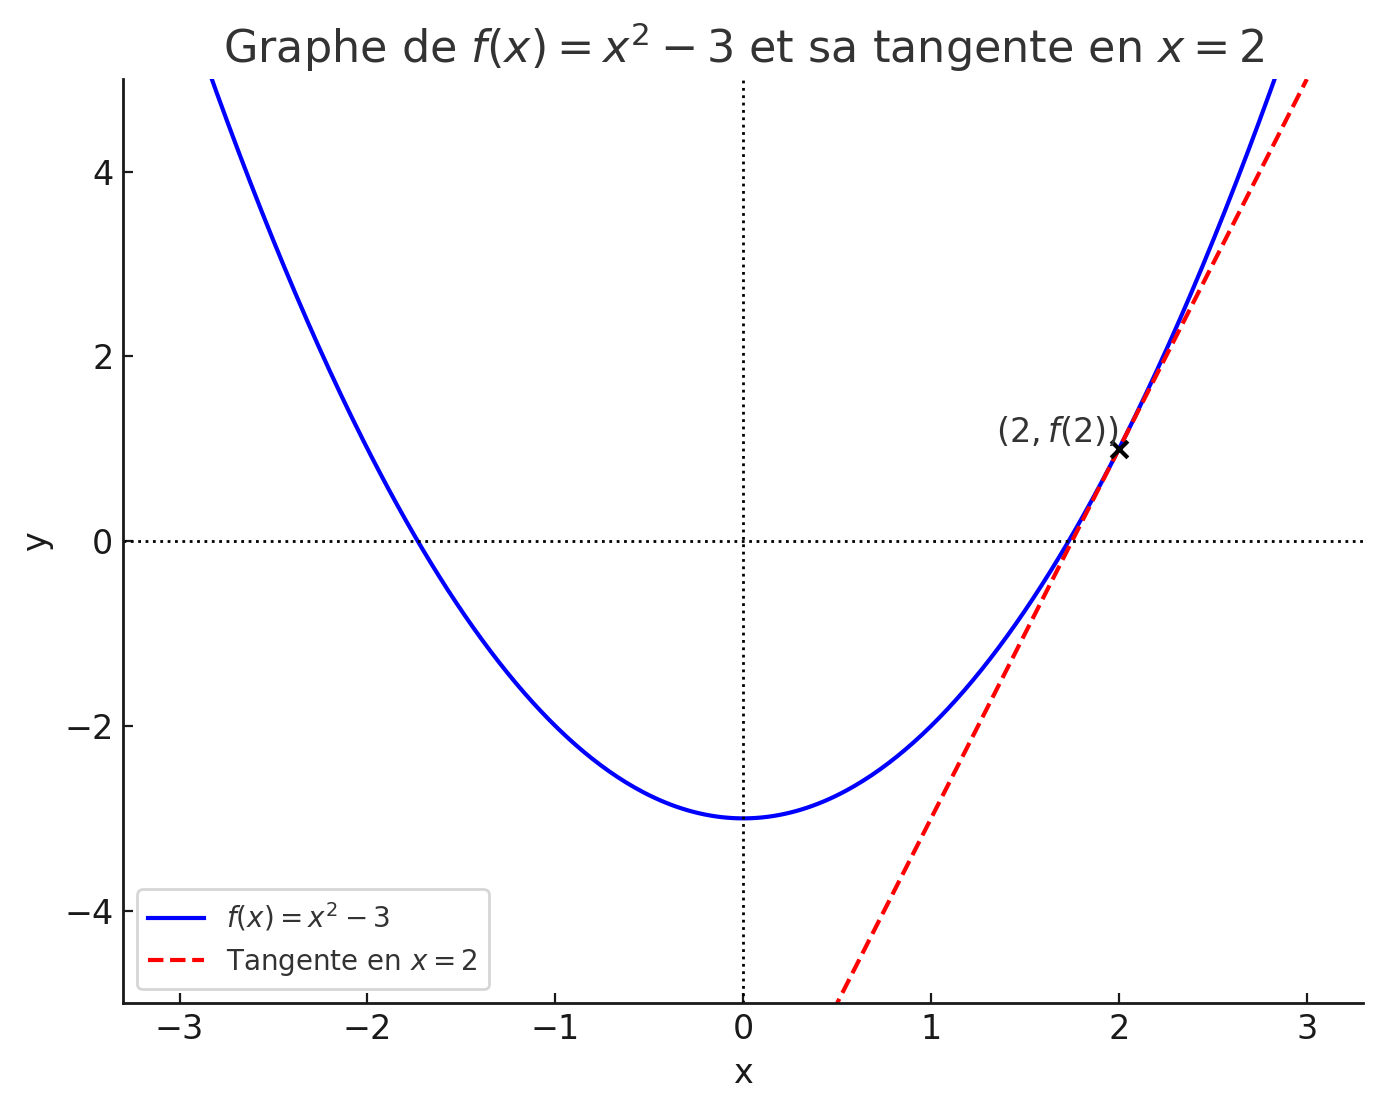
\includegraphics[width=0.5\textwidth]{graphe2.png}
    \end{center}
\end{solution}
}{}
\item Donner l'équation de la tangente à $f$ en $x=2$. 

\ifthenelse{\boolean{showSolutions}}{
\begin{solution}
    \begin{align*}
        y = f'(2)(x-2) + f(2)
    \end{align*}
    C'est à dire $y = 4x - 7$.
\end{solution}
}{}
\item Donner l'expression du point $x_1$ intersection de la tangente à $f$ en $x=2$ avec l'axe des abscisses. 

\ifthenelse{\boolean{showSolutions}}{
\begin{solution}
    \begin{align*}
        x_1 = \frac{7}{4}
    \end{align*}
\end{solution}
}{}
\item En déduire une valeur approchée de $\sqrt{3}$ en partant de $x_0 = 2$ et en appliquant une fois la méthode de Newton. \newline
\noindent Quelle erreur commet-on ?

\ifthenelse{\boolean{showSolutions}}{
\begin{solution}
    $x_1 = \frac{7}{4} \approx 1.75$.
    L'erreur commise est de $|\sqrt{3}-1.75| \approx 0.02$.

    L'erreur relative est de $0.02/\sqrt{3} \approx 1\%$.
\end{solution}
}{}

\item Rédiger un pseudo-code pour implémenter la méthode de Newton. 

\ifthenelse{\boolean{showSolutions}}{
\begin{solution}
        x = 2

        Tant que |f(x)| > 1e-10:

        \hspace{2em}  x = x - f(x)/f'(x)

        Afficher x
\end{solution}
}{}

\vspace{1em}
Le théorème de Taylor-Lagrange donne que pour toute fonction de classe $\mathbb{C}^2$ sur un intervalle $[a,b]$ et pour tout $c\in[a,b]$,
\[
    \Big|f(c)-\big(f(x)+f'(x)(c-x)\big)\Big| \leq \frac{\max_{x\in[a,b]}|f''(x)|}{2!}|x-c|^2
\]

\item En appliquant l'inégalité avec $x=x_n$, déterminez une constante $k$ telle que 
\[
\left|x_{n+1}-\gamma\right| \leq k\left|x_n-\gamma\right|^2\,.
\]
\noindent \textit{On dira que la convergence de la suite est quadratique.}

\ifthenelse{\boolean{showSolutions}}{
\begin{solution}
    On applique l'inégalité avec $x=x_n$ et $c=\sqrt{3}$.
    \[
        \left|-f\left(x_n\right)-f^{\prime}\left(x_n\right)\left(\sqrt{3}-x_n\right)\right| \leq \frac{1}{2} \max _{[a, b]}\left|f^{\prime \prime}\right|\left|x_n-\sqrt{3}\right|^2
    \]
    En divisant par $f'(x_n)$ qui est non nul on obtient
    \[
    \left|x_{n+1}-\gamma\right| \leq \frac{\max _{[a, b]}\left|f^{\prime \prime}\right|}{2\left|f^{\prime}\left(x_n\right)\right|}\left|x_n-\gamma\right|^2 \leq \frac{1}{2} \frac{\max _{[a, b]}\left|f^{\prime \prime}\right|}{\min _{[a, b]}\left|f^{\prime}\right|}\left|x_n-\gamma\right|^2\,.
    \]

    Comme $|f''|<2$ et $|f'|\geq 3.4$ on obtient
    \[
        \left|x_{n+1}-\sqrt{3}\right| \leq  \frac{1}{3.4}\left|x_n-\sqrt{3}\right|^2\,.
    \]
\end{solution}
}{}

\item Montrer que 
\[
k\left|x_{n+1}-\gamma\right| \leq \left(k\left|x_0-\gamma\right|\right)^{2^{n+1}}
\]
\item Combien d'itérations de la méthode de Newton sont nécessaires pour approcher $\sqrt{3}$ à $10^{-20}$ près ?

\ifthenelse{\boolean{showSolutions}}{
\begin{solution}
$$
\begin{aligned}
\frac{1}{k \times 34^{2^n}} \leq 10^{-20} & \Longleftrightarrow \frac{10^{20}}{k} \leq 34^{2^n} \\
& \Longleftrightarrow \ln \left(\frac{10^{20}}{k}\right) \leq 2^n \ln 34 \\
& \Longleftrightarrow \frac{1}{\ln 2} \ln \left(\frac{\ln \left(\frac{10^{20}}{k}\right)}{\ln 34}\right) \leq n .
\end{aligned}
$$


La valeur $n=4$ convient, ce qui est plutôt rapide :) 
\end{solution}
}{}

\end{enumerate}

\vspace{3cm}
\section*{Polynômes de Lagrange}
On cherche à approcher la fonction $\exp$ par un polynôme. 
\begin{enumerate}
    \item Si on fixe $3$ points du plan, quel est au minimum le degré d'un polynôme qui passe par ces $3$ points ? 

    \ifthenelse{\boolean{showSolutions}}{
    \begin{solution}
        Au moins de degré $2$
    \end{solution}
    }{}
    \item Donner un polynôme $\ell_0$ qui vaut $1$ en $0$ et $0$ aux points $1$ et $2$. \newline
    \noindent \textit{On pourra aller consulter le cm avant de regarder la solution.}

    \ifthenelse{\boolean{showSolutions}}{
    \begin{solution}
        $\ell_0$ est un polynôme de degré $2$ qui vaut $0$ aux points $1$ et $2$. $\ell_0$ admet donc deux racines : $1$ et $2$. 
        On peut donc écrire $\ell_0(x) = a(x-1)(x-2)$. 
        On sait que $\ell_0(0) = 1$ donc $a = \frac{1}{2}$. 
        On obtient $\ell_0(x) = \frac{1}{2}(x-1)(x-2)$.
    \end{solution}
    }{}
    \item Donne de même un polynôme $\ell_1$ qui passe par les points $(0,0), (1, 1), (2, 0)$ et un polynôme $\ell_2$ qui passe par les points $(0,0), (1, 0), (2, 1)$ 
    
\ifthenelse{\boolean{showSolutions}}{
\begin{solution}
    On construit de même $\ell_1$ et $\ell_2$ tels que 
    \begin{itemize}
        \item $\ell_1$ vaut $1$ en $1$ et $0$ en $0$ et $2$
        \item $\ell_2$ vaut $1$ en $2$ et $0$ en $0$ et $1$
    \end{itemize}
    On obtient 
    \[
    \ell_1(x) = - x(x-2)
    \]
    et 
    \[
    \ell_2(x) = \frac{1}{2}\, x(x-1)
    \]
\end{solution}
}{}
    
\item Donner un polynôme $P_2$ qui passe par les points $(0,1)$, $(1,e)$ et $(2,e^2)$. 

\ifthenelse{\boolean{showSolutions}}{
\begin{solution}
On va chercher $P_2$ comme une somme pondérée des polynômes $\ell_0$, $\ell_1$ et $\ell_2$, Si on écrit

\[
    P_2(x) = \alpha\cdot \ell_0(x) + \beta\cdot \ell_1(x) + \gamma\cdot \ell_2(x)
    \]
    alors, seul $\alpha$ compte pour la valeur de $P_2$ en $0$. 
    La valeur de $\beta$ est la seule à compter pour $P_2(1)$ et $\gamma$ est la seule à compter pour $P_2(2)$. 
    
    On pose 
    \[
    P_2(x) = 1\cdot \ell_0(x) + e\cdot \ell_1(x) + e^2\cdot \ell_2(x)
    \]
\end{solution}
}{}

\item Avec une calculatrice ou \url{desmos.com}, tracer le graphe de $P_2$ et de $\exp$ sur l'intervalle $[0,2]$. 

\ifthenelse{\boolean{showSolutions}}{
\begin{solution}
    \begin{center}
        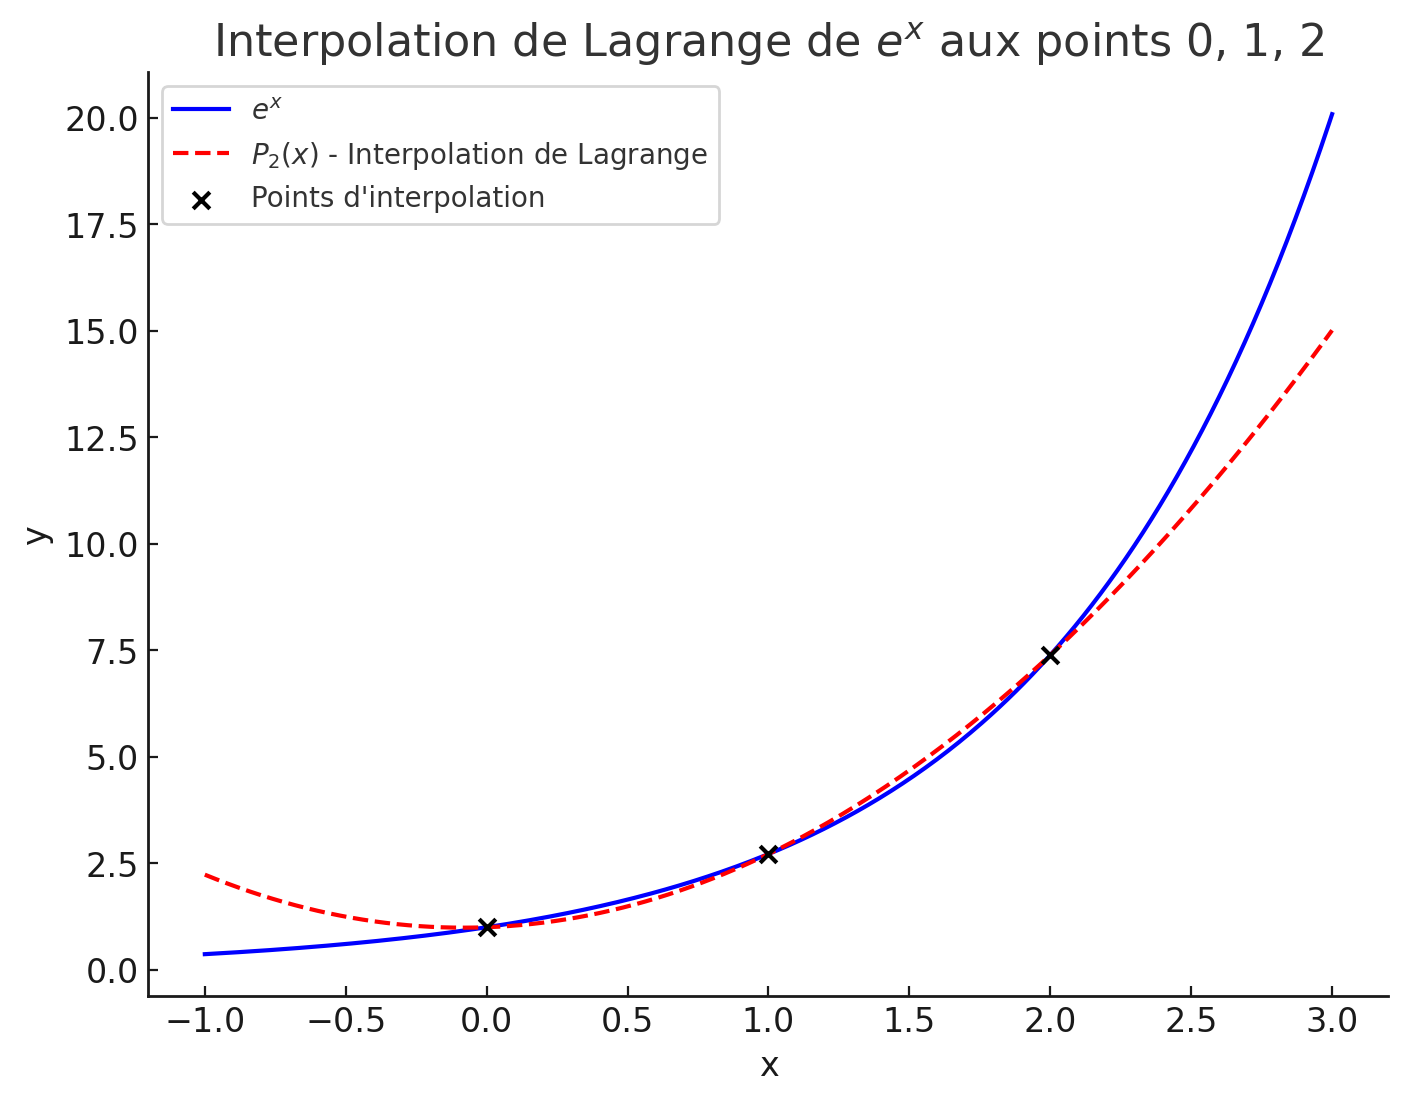
\includegraphics[width=0.5\textwidth]{graphe3.png}
    \end{center}
\end{solution}
}{}

\item Donner une valeur approchée de $e^{0.5}$ en utilisant $P_2$, et aussi de $e^{10}$. Calculer les erreurs commises.  

\ifthenelse{\boolean{showSolutions}}{
\begin{solution}
    $P_2(0.5) \approx 1.49$ et $e^{0.5} \approx 1.65$. L'erreur absolue est de $0.16$ et l'erreur relative d'environ $10\%$.

    $P_2(10) \approx 151$ alors que $e^{10} \approx 22\, 000$. L'erreur absolue est de $21\, 850$ et l'erreur relative de presque $100\%$.
\end{solution}
}{}

\item Rédiger un pseudo-code pour calculer $P_n$, un polynôme qui coïncide avec $\exp$ sur les $n+1$ premiers entiers. 

\ifthenelse{\boolean{showSolutions}}{
\begin{solution}
Par exemple, pour calculer le $k$-ième polynôme $\ell_k$ : 

    fonction $l_k$ : 

    base = 1

    Pour j qui prend toutes les valeurs de 0 à n:

     \hspace{2em}   Si $j \neq k$:

            \hspace{2em}\hspace{2em}   base $*= (x - j) / (k - j)$

    return base


on peut ensuite définir le polynôme $P_n$ :

    fonction Pn : 

    P = 0

    Pour i qui prend toutes les valeurs de 0 à n:

        \hspace{2em}   $P += \exp(i) * l_k$

    return P

\end{solution}
}{}

\end{enumerate}


\end{document}
